\begin{recipe}
    [% 
        preparationtime = {\unit[30]{min}},
        bakingtime = {\unit[1]{h}},
        portion = {\portion{6-8}},
        source = {polish wisdom}
    ]
    {Strawberry cake}

    \ingredients[14]{%
        \textbf{Sponge} & \\
        5 & eggs \\
        \unit[3/4]{c} & Sugar \\
        \unit[3/4]{c} & Flour \\
        \unit[\nicefrac{1}{4}]{c} & Starch (Potato or corn) \\
        \textbf{Cream} & \\
        \unit[3]{c} & Milk \\
        \unit[3/4]{c} & Sugar \\
        \unit[4]{tbs.} & Flour \\
        \unit[4]{tbs.} & Starch \\
        \unit[150-250]{g} & Butter \\
        1 & Egg yolk
    }

    \preparation{%
        \step All ingredients for sponge must be at room temperature.
        Beat whites until stiff.
        While still beating, add sugar (one spoon at the time).
        Then egg yolks (one at the time, beating gently).
        \step Add sifted flour. \underline{Don't beat.} Gently mix with a spatula.
        \step Line the cake tin with parchment (only bottom), don't grease sides.
        Fill with batter.
        \underline{Bake at \unit[160-170]{\textcelcius} for 35-40min.}
        \step Boil 2/3 milk and sugar up.
        In a cup or high blender dish mix (with fork or a beater) flour, yolk and remaining milk.
        When sugar/milk liquid is boiling, add flour/milk and stir vigorously for about 2 min.
        Remove from heating and continue stirring.
        \step Cool the blancmange (step 4).
        Cream butter and mix with blancmange (add in small portions).
        \step Sandwich the sponge and decorate with fresh fruit!
    }

    \suggestion[Spice it up!]
    {%
        To make chocolate cream, add cocoa powder to milk-flour mixture.
    }

    \hint{%
        Drop hot sponge in the tin on the kitchen bench/floor from 30cm.
        Trust me, it will keep the cake fluffier.
    }

\end{recipe}

\begin{figure}[h]
    \centering
    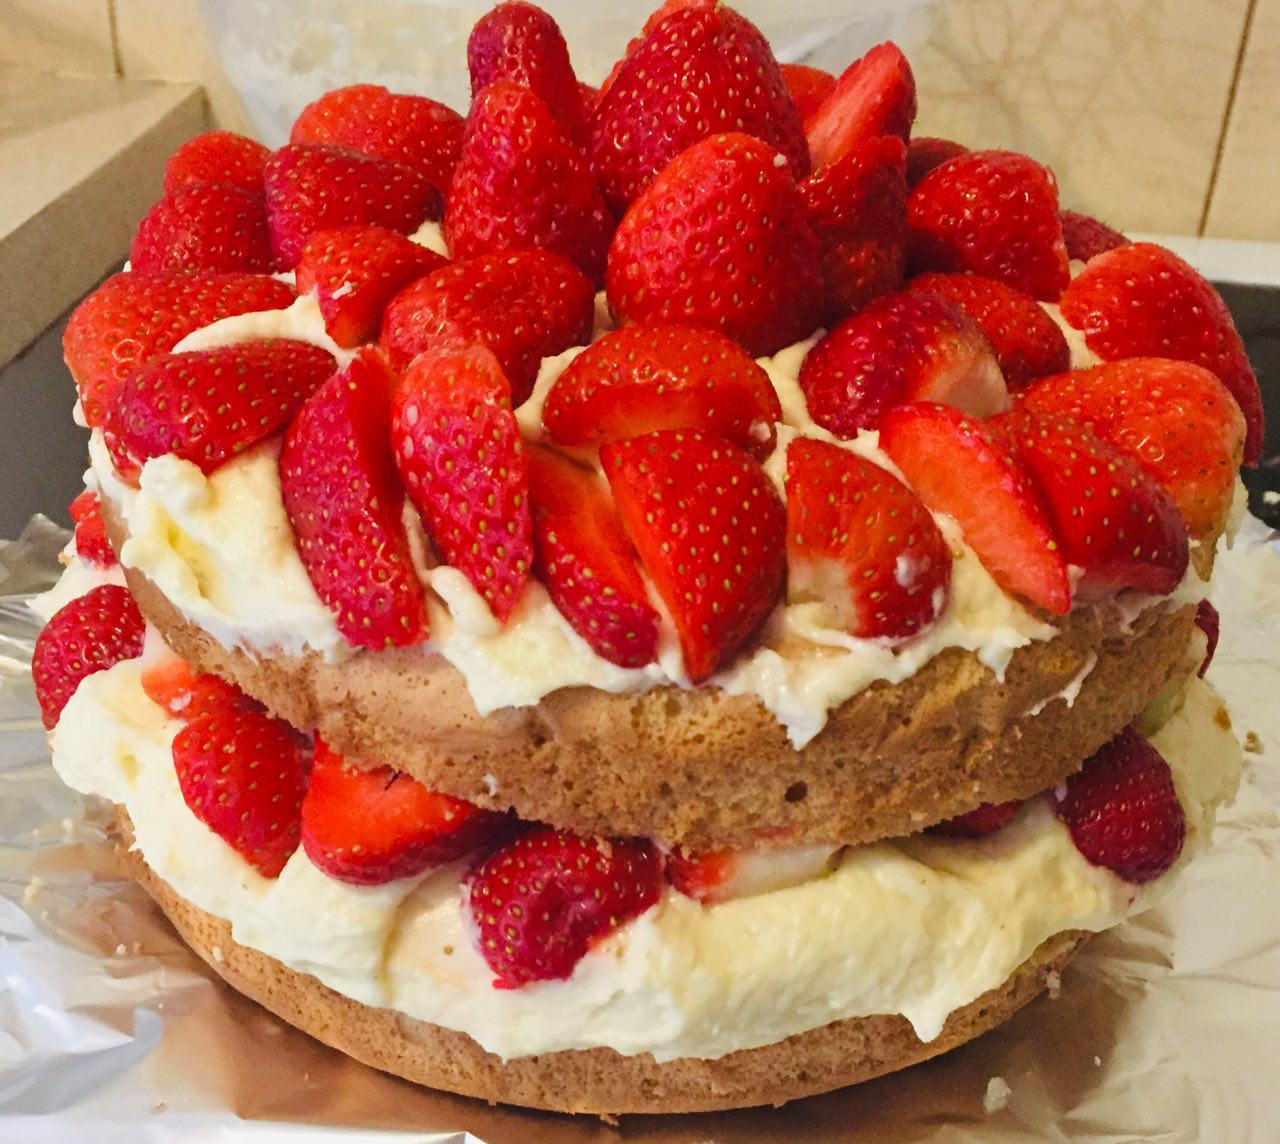
\includegraphics[width=8cm]{pic/strawberry_cake}
\end{figure}
